
%(BEGIN_QUESTION)
% Copyright 2015, Tony R. Kuphaldt, released under the Creative Commons Attribution License (v 1.0)
% This means you may do almost anything with this work of mine, so long as you give me proper credit

Determine the statuses of all lamps and relay coils in this circuit, given the following process conditions:

$$\includegraphics[width=15.5cm]{i01087x01.eps}$$

\begin{itemize}
\item{} Flow = 3.5 GPM
\item{} Pressure = 41 PSI
\item{} Temperature = 155 $^{o}$F
\item{} Level = 1.3 ft
\item{} Pushbutton A = {\it unpressed}
\item{} Pushbutton B = {\it unpressed}
\end{itemize}

\underbar{file i01087}
%(END_QUESTION)





%(BEGIN_ANSWER)

\noindent
{\bf Fully annotated circuit schematic:}  {\it ``X'' representing an open contact or de-energized load, and ``'' representing a closed contact or energized load}

$$\includegraphics[width=15.5cm]{i01087x02.eps}$$

Recall that a process switch will be in its resting (``normal'') condition when the stimulus value is less than the trip threshold, and will be in its actuated condition when the stimulus exceeds the threshold.

\vskip 10pt

Therefore,
 
\begin{itemize}
\item{} CR1 coil = {\bf de-energized}
\item{} Blue lamp = {\bf energized}
\item{} Red lamp = {\bf de-energized}
\item{} Amber lamp = {\bf energized} 
\end{itemize}

%(END_ANSWER)





%(BEGIN_NOTES)

%INDEX% Switch, pressure: ladder logic circuit

%(END_NOTES)


